\chapter{Text \& Sentiment Analysis}

\section{Pengantar Text \& Sentiment Analysis}

Analisis teks (\textit{text analysis}) merupakan cabang dari \textit{Natural Language Processing} (NLP) yang berfokus pada pengolahan, ekstraksi informasi, dan penemuan pola dari data berbasis teks. Sumber data teks dapat sangat beragam, mulai dari ulasan pelanggan di platform e-commerce, komentar media sosial, email, forum diskusi, hingga berita dan dokumen internal perusahaan. Tujuan utamanya adalah mengubah informasi yang tidak terstruktur menjadi data terstruktur yang dapat dianalisis lebih lanjut untuk mendukung pengambilan keputusan \cite{cambria2017sentiment}. 

Salah satu bidang penting dalam analisis teks adalah analisis sentimen (\textit{sentiment analysis}) atau sering juga disebut \textit{opinion mining}. Bidang ini bertujuan untuk mengidentifikasi, mengukur, dan mengklasifikasikan opini, sikap, atau emosi yang terkandung dalam sebuah teks \cite{liu2012sentiment}. Analisis sentimen dapat menghasilkan kategori seperti positif, negatif, atau netral, maupun skor numerik yang menunjukkan intensitas sentimen, misalnya dalam rentang -1 hingga +1. Dalam praktiknya, analisis dapat dilakukan pada tingkat dokumen untuk mengetahui sentimen keseluruhan, pada tingkat kalimat untuk menilai setiap pernyataan, atau bahkan pada tingkat aspek untuk mengidentifikasi sentimen terhadap bagian tertentu dari objek yang dibahas, seperti pada ulasan yang menyebutkan “pelayanannya cepat tetapi makanannya hambar”.

Relevansi analisis teks dan sentimen dalam dunia bisnis sangat tinggi. Perusahaan dapat memahami persepsi publik terhadap merek mereka secara real-time, mendeteksi masalah layanan sebelum berkembang menjadi krisis reputasi, mengukur efektivitas kampanye pemasaran, serta mengidentifikasi tren atau isu yang sedang berkembang di pasar. Contohnya, analisis sentimen pada media sosial dapat membantu perusahaan ritel menentukan strategi promosi yang lebih tepat sasaran, sementara di sektor keuangan, analisis ini dapat dimanfaatkan untuk memantau opini pasar sebagai dasar pengambilan keputusan investasi.

Pendekatan untuk melakukan analisis sentimen dapat bervariasi. Metode berbasis leksikon menggunakan kamus kata yang telah diberikan skor sentimen, sementara metode berbasis pembelajaran mesin melatih model klasifikasi seperti \textit{Naive Bayes}, \textit{Logistic Regression}, atau SVM untuk mengenali pola sentimen. Lebih lanjut, perkembangan \textit{deep learning} telah memungkinkan pemodelan yang lebih kontekstual dengan memanfaatkan arsitektur seperti LSTM atau model berbasis \textit{transformer} (misalnya BERT dan RoBERTa) yang mampu memahami hubungan kata dalam konteks yang lebih luas \cite{yang2019xlnet}.

Meski demikian, analisis sentimen memiliki tantangan tersendiri. Ambiguitas bahasa, sarkasme, dan ironi seringkali sulit diidentifikasi, terutama oleh model sederhana. Fenomena \textit{code-switching} atau penggunaan campuran bahasa dalam satu teks juga menjadi hambatan, begitu pula dengan sifat ketergantungan domain di mana model yang dilatih pada satu topik atau industri belum tentu efektif saat diterapkan pada domain lain. Tantangan-tantangan ini mendorong peneliti dan praktisi untuk terus mengembangkan metode yang lebih adaptif dan akurat.

Dengan memahami dasar-dasar ini, pembaca akan lebih siap untuk mengeksplorasi implementasi praktis analisis teks dan sentimen menggunakan alat bantu visual seperti Orange, yang akan dibahas pada bagian selanjutnya.


\section{Aplikasi Bisnis Text \& Sentiment Analysis}

Penerapan analisis teks dan sentimen dalam dunia bisnis telah berkembang pesat seiring meningkatnya volume data tidak terstruktur yang dihasilkan setiap hari, terutama dari media sosial, platform ulasan, dan interaksi layanan pelanggan. Dengan memanfaatkan teknik ini, perusahaan dapat mengubah aliran informasi yang masif menjadi wawasan strategis yang dapat memengaruhi keputusan bisnis secara langsung.

Dalam sektor e-commerce, analisis sentimen digunakan untuk memahami persepsi pelanggan terhadap produk atau merek. Ulasan dan komentar pembeli dianalisis untuk mengidentifikasi kekuatan dan kelemahan produk, memberikan gambaran yang lebih akurat dibandingkan sekadar mengandalkan angka penjualan. Misalnya, sebuah toko daring dapat menemukan bahwa meskipun sebuah produk terjual dengan baik, banyak pelanggan mengeluhkan kualitas kemasannya. Informasi ini dapat mendorong perbaikan produk atau layanan pasca-penjualan.

Industri perbankan dan keuangan memanfaatkan analisis teks untuk memantau opini publik dan sentimen pasar terhadap lembaga keuangan, instrumen investasi, atau kebijakan moneter. Data dari forum investor, berita ekonomi, dan media sosial dapat memberikan sinyal awal tentang perubahan kepercayaan pasar. Dengan memahami perubahan sentimen ini, manajer investasi dapat menyesuaikan strategi portofolio mereka lebih cepat daripada jika hanya mengandalkan data keuangan konvensional.

Di sektor pariwisata dan perhotelan, analisis sentimen berperan penting dalam memantau ulasan destinasi wisata dan akomodasi. Hotel dapat memanfaatkan informasi ini untuk mengidentifikasi aspek layanan yang paling dihargai oleh tamu, seperti kebersihan kamar atau keramahan staf, sekaligus menemukan area yang perlu ditingkatkan. Hal ini tidak hanya meningkatkan kepuasan pelanggan, tetapi juga membantu membangun reputasi positif secara berkelanjutan.

Sektor ritel fisik dan daring dapat menggunakan analisis teks untuk memahami tren konsumen dan preferensi produk. Data dari media sosial, misalnya, dapat menunjukkan lonjakan minat terhadap suatu kategori produk tertentu, bahkan sebelum tren tersebut tercermin dalam data penjualan. Dengan demikian, pengecer dapat mengoptimalkan persediaan dan kampanye pemasaran sesuai dengan permintaan yang sedang berkembang.

Pemerintah dan lembaga publik juga memanfaatkan analisis sentimen untuk mengukur reaksi masyarakat terhadap kebijakan tertentu. Melalui pemantauan opini publik di media sosial dan portal berita, pembuat kebijakan dapat menilai tingkat penerimaan masyarakat, mengidentifikasi potensi resistensi, dan menyesuaikan pendekatan komunikasi mereka untuk meningkatkan efektivitas implementasi kebijakan.

Penggunaan analisis teks dan sentimen dalam bisnis tidak hanya sebatas memahami kondisi saat ini, tetapi juga bersifat prediktif. Dengan menggabungkan data historis dan analisis tren, perusahaan dapat mengantisipasi perubahan perilaku konsumen dan mengembangkan strategi yang lebih proaktif. Pendekatan ini menjadikan analisis teks dan sentimen sebagai salah satu pilar penting dalam manajemen berbasis data modern, di mana kecepatan dan ketepatan informasi menjadi keunggulan kompetitif yang signifikan.


\section{Teknik dan Metode Populer}

Berbagai pendekatan telah dikembangkan untuk melakukan analisis teks dan sentimen, masing-masing dengan karakteristik, kelebihan, dan keterbatasannya. Tiga pendekatan yang paling umum digunakan adalah metode berbasis kamus, berbasis pembelajaran mesin, dan berbasis pembelajaran mendalam. Pemilihan metode yang tepat biasanya mempertimbangkan faktor seperti ketersediaan data berlabel, kebutuhan akurasi, dan sumber daya komputasi yang tersedia.

\subsection{Analisis Berbasis Kamus (Lexicon-based Approach)}

Pendekatan berbasis kamus memanfaatkan daftar kata atau frasa yang telah dilengkapi dengan nilai sentimen, baik positif maupun negatif. Nilai ini dapat berupa skor numerik atau label kategorikal yang menunjukkan tingkat kekuatan sentimen. Proses analisis dilakukan dengan mencocokkan kata-kata dalam teks dengan entri yang ada di kamus, lalu menghitung skor keseluruhan berdasarkan kemunculan dan bobot kata-kata tersebut.

Kelebihan metode ini terletak pada kesederhanaannya dan kemampuannya bekerja tanpa memerlukan data berlabel yang besar. Oleh karena itu, metode ini sering digunakan dalam skenario di mana dataset pelatihan tidak tersedia atau sangat terbatas. Namun, kelemahannya cukup signifikan, terutama dalam menghadapi ambiguitas makna, sarkasme, dan konteks yang kompleks. Sebagai contoh, kalimat “Layanannya luar biasa cepat, sampai saya tidak sempat duduk” mungkin memiliki kata-kata positif secara leksikal, tetapi konteksnya bisa menyiratkan keluhan.

Contoh sumber kamus sentimen yang populer antara lain SentiWordNet, AFINN, dan VADER (\textit{Valence Aware Dictionary and sEntiment Reasoner}) yang dirancang khusus untuk teks informal seperti media sosial.

\subsection{Analisis Berbasis Machine Learning}

Pendekatan berbasis pembelajaran mesin menggunakan algoritma klasifikasi untuk membangun model yang dapat mengenali pola sentimen dari data berlabel. Tahapannya meliputi pengumpulan dataset, prapemrosesan teks (seperti tokenisasi, normalisasi, dan penghapusan kata umum), ekstraksi fitur (misalnya dengan metode \textit{bag-of-words} atau TF-IDF), pelatihan model, dan evaluasi performa.

Algoritma yang sering digunakan mencakup \textit{Naive Bayes}, \textit{Logistic Regression}, \textit{Support Vector Machines} (SVM), dan \textit{Random Forest}. Metode ini memiliki keunggulan dalam kemampuan belajar dari data domain-spesifik dan menyesuaikan bobot fitur berdasarkan konteks. Dengan data pelatihan yang memadai, model dapat mencapai akurasi tinggi dan adaptif terhadap variasi bahasa.

Namun, pendekatan ini memerlukan dataset yang cukup besar dan representatif untuk dapat bekerja dengan baik. Selain itu, model yang dihasilkan dapat mengalami penurunan performa ketika diterapkan pada domain yang berbeda dari data pelatihannya, sehingga memerlukan proses pelatihan ulang atau penyesuaian domain.

\subsection{Analisis Berbasis Deep Learning}

Pendekatan berbasis pembelajaran mendalam memanfaatkan arsitektur jaringan saraf tiruan yang kompleks untuk memahami representasi kata dan konteks secara lebih mendalam. Metode ini tidak hanya mengandalkan frekuensi kata, tetapi juga mampu menangkap hubungan semantik dan sintaksis di antara kata-kata dalam sebuah teks.

Arsitektur yang umum digunakan meliputi Long Short-Term Memory (LSTM) dan Gated Recurrent Unit (GRU) untuk menangani data sekuensial, Convolutional Neural Networks (CNN) untuk ekstraksi fitur lokal, serta model berbasis \textit{transformer} seperti BERT, RoBERTa, dan XLNet yang memanfaatkan mekanisme \textit{self-attention} untuk memahami konteks secara global \cite{yang2019xlnet}.

Kelebihan utama metode ini adalah kemampuannya mencapai akurasi yang sangat tinggi, bahkan dalam menghadapi bahasa yang kompleks dan kontekstual. Selain itu, model \textit{pre-trained} yang tersedia secara publik dapat diadaptasi (\textit{fine-tuning}) untuk berbagai domain dengan jumlah data yang relatif lebih sedikit. Kekurangannya adalah kebutuhan komputasi yang tinggi dan waktu pelatihan yang lebih lama, sehingga implementasinya memerlukan perangkat keras yang memadai atau layanan komputasi awan.

Dalam praktiknya, pilihan antara ketiga pendekatan ini sering kali melibatkan pertimbangan keseimbangan antara ketersediaan data, sumber daya komputasi, dan kebutuhan akurasi. Tidak jarang, praktisi menggabungkan beberapa pendekatan dalam sebuah sistem hibrid untuk memanfaatkan keunggulan masing-masing metode.


\section{Alur Proses Text \& Sentiment Analysis}

Proses analisis teks dan sentimen tidak dapat dilakukan secara instan, melainkan memerlukan tahapan yang sistematis agar hasil yang diperoleh akurat dan relevan. Alur ini dimulai dari pengumpulan data teks, dilanjutkan dengan serangkaian langkah prapemrosesan, hingga ke tahap ekstraksi fitur dan pemodelan. Pada bagian ini, fokus akan diberikan pada dua tahapan awal yang sangat menentukan kualitas analisis, yaitu pengumpulan data dan prapemrosesan teks.

\subsection{Pengumpulan Data Teks}

Pengumpulan data merupakan langkah pertama dan paling mendasar dalam analisis teks dan sentimen. Data teks dapat berasal dari berbagai sumber, baik internal maupun eksternal. Sumber internal meliputi email pelanggan, formulir umpan balik, transkrip layanan pelanggan, dan catatan internal perusahaan. Sementara itu, sumber eksternal mencakup ulasan produk di situs e-commerce, komentar di media sosial, forum diskusi, blog, berita daring, dan dataset publik yang disediakan oleh lembaga penelitian atau komunitas.

Metode pengumpulan data dapat dilakukan secara manual atau otomatis. Untuk data yang tersedia dalam format terstruktur seperti CSV atau database, prosesnya relatif sederhana. Namun, untuk data yang tersebar di internet, pengambilan dapat dilakukan melalui \textit{web scraping} menggunakan pustaka seperti \texttt{BeautifulSoup} atau \texttt{Scrapy}, atau dengan memanfaatkan API resmi dari platform seperti Twitter, Reddit, atau Google Reviews. Penggunaan dataset publik juga menjadi pilihan populer, misalnya \textit{Sentiment Labelled Sentences} dari UCI Machine Learning Repository yang berisi kalimat ulasan dari Amazon, Yelp, dan IMDB yang sudah diberi label sentimen positif atau negatif.

Kualitas data yang dikumpulkan sangat mempengaruhi performa model. Data yang bias, tidak representatif, atau terlalu sedikit dapat menghasilkan model yang kurang akurat. Oleh karena itu, selain kuantitas, aspek keberagaman dan keseimbangan kelas sentimen (misalnya jumlah data positif dan negatif yang seimbang) perlu diperhatikan.

\subsection{Preprocessing Teks}

Setelah data terkumpul, tahap berikutnya adalah prapemrosesan atau \textit{text preprocessing}, yaitu proses membersihkan dan menyiapkan data teks agar dapat diolah oleh algoritma analisis. Teks mentah sering kali mengandung elemen yang tidak relevan seperti tanda baca, angka, URL, atau simbol khusus, yang dapat mengganggu proses analisis jika tidak dihilangkan.

Langkah prapemrosesan umumnya mencakup beberapa proses utama. Pertama, \textit{tokenisasi} memisahkan teks menjadi unit-unit kata atau frasa. Kedua, normalisasi teks dilakukan untuk menyeragamkan format, misalnya mengubah semua huruf menjadi huruf kecil, menghapus tanda baca, dan memperbaiki ejaan yang tidak konsisten. Ketiga, \textit{stopword removal} menghapus kata-kata umum yang tidak memiliki kontribusi signifikan terhadap makna, seperti “dan”, “atau”, “yang”. Selanjutnya, \textit{stemming} atau \textit{lemmatization} digunakan untuk mengubah kata menjadi bentuk dasarnya, sehingga kata “berlari” dan “berlarian” diperlakukan sebagai kata yang sama.

Selain itu, pada teks yang berasal dari media sosial, penanganan elemen khusus seperti emotikon, \textit{hashtag}, dan \textit{mentions} juga perlu dilakukan, karena elemen-elemen tersebut dapat memuat informasi sentimen yang penting. Misalnya, emotikon “😊” umumnya memiliki konotasi positif, sedangkan “😡” cenderung negatif.

Tahap prapemrosesan yang baik akan menghasilkan representasi teks yang bersih dan konsisten, sehingga memudahkan proses ekstraksi fitur pada tahap berikutnya. Tanpa prapemrosesan yang memadai, model analisis sentimen berisiko mengalami penurunan performa akibat kebisingan (\textit{noise}) dalam data.

\subsection{Ekstraksi Fitur}

Ekstraksi fitur adalah proses mengubah teks yang telah dipraproses menjadi representasi numerik yang dapat dipahami oleh algoritma pembelajaran mesin. Hal ini penting karena sebagian besar algoritma analisis tidak dapat langsung memproses data dalam bentuk teks mentah. Representasi numerik ini berfungsi sebagai deskripsi karakteristik teks, di mana setiap dokumen atau kalimat direpresentasikan oleh vektor angka yang mencerminkan keberadaan, frekuensi, atau makna kata-kata yang dikandungnya.

Salah satu metode yang paling sederhana adalah \textit{Bag-of-Words} (BoW), di mana setiap kata unik dalam korpus menjadi sebuah fitur, dan nilainya adalah jumlah kemunculan kata tersebut dalam dokumen. Meskipun mudah diterapkan, metode ini mengabaikan urutan kata dan konteks. Untuk mengatasi keterbatasan ini, digunakan pendekatan \textit{Term Frequency–Inverse Document Frequency} (TF-IDF) yang memberikan bobot lebih tinggi pada kata-kata yang sering muncul di dokumen tertentu tetapi jarang muncul di keseluruhan korpus. Hal ini membantu menyoroti kata-kata yang lebih bermakna secara kontekstual.

Perkembangan terbaru dalam NLP memperkenalkan teknik representasi berbasis \textit{word embeddings}, seperti Word2Vec, GloVe, dan FastText, yang memetakan kata-kata ke dalam ruang vektor berdimensi rendah sehingga kata-kata dengan makna serupa memiliki representasi yang berdekatan. Lebih lanjut, model \textit{contextual embeddings} seperti BERT dan RoBERTa mampu menghasilkan representasi kata yang bergantung pada konteks kalimat, sehingga kata “bank” pada kalimat “saya menyimpan uang di bank” akan memiliki vektor yang berbeda dengan “bebek itu berdiri di tepi bank sungai”.

Pemilihan teknik ekstraksi fitur yang tepat sangat bergantung pada tujuan analisis, ukuran dataset, dan sumber daya komputasi yang tersedia. Pendekatan sederhana seperti TF-IDF sering cukup efektif untuk tugas klasifikasi sentimen dasar, sementara \textit{contextual embeddings} lebih unggul pada tugas yang memerlukan pemahaman mendalam terhadap konteks bahasa.

\subsection{Klasifikasi Sentimen}

Tahap klasifikasi sentimen bertujuan untuk memetakan representasi numerik dari teks ke dalam kategori sentimen, seperti positif, negatif, atau netral. Proses ini dilakukan dengan melatih model klasifikasi menggunakan dataset berlabel yang telah diekstraksi fiturnya.

Algoritma yang digunakan untuk klasifikasi sentimen sangat bervariasi, mulai dari metode tradisional seperti \textit{Logistic Regression}, \textit{Naive Bayes}, dan Support Vector Machines (SVM), hingga metode ansambel seperti Random Forest dan Gradient Boosting. Pada tingkat yang lebih canggih, digunakan arsitektur pembelajaran mendalam seperti LSTM, GRU, atau model berbasis \textit{transformer} yang mampu memahami dependensi jangka panjang dan hubungan kompleks antar kata.

Proses pelatihan melibatkan pembagian dataset menjadi subset pelatihan dan pengujian, serta penyesuaian parameter model untuk meminimalkan kesalahan prediksi. Dalam kasus tertentu, data juga dibagi menjadi subset validasi untuk mengoptimalkan hiperparameter dan mencegah \textit{overfitting}.

Output dari model ini dapat berupa label kategorikal atau skor probabilitas. Misalnya, sebuah ulasan dapat diberi label “positif” dengan probabilitas 0,85, yang menunjukkan keyakinan model terhadap klasifikasi tersebut.

\subsection{Evaluasi Model}

Evaluasi model merupakan langkah penting untuk menilai sejauh mana model klasifikasi sentimen bekerja dengan baik. Pemilihan metrik evaluasi harus disesuaikan dengan tujuan analisis dan distribusi kelas pada dataset. Metrik yang paling umum digunakan adalah akurasi, yang mengukur proporsi prediksi yang benar dibandingkan dengan total prediksi. Namun, pada dataset yang tidak seimbang (misalnya jumlah data positif jauh lebih banyak daripada negatif), akurasi saja seringkali menyesatkan.

Oleh karena itu, metrik lain seperti presisi, recall, dan F1-score sering digunakan untuk memberikan gambaran yang lebih seimbang tentang performa model. Presisi mengukur seberapa banyak prediksi positif yang benar-benar positif, sementara recall mengukur seberapa banyak kasus positif yang berhasil terdeteksi oleh model. F1-score merupakan rata-rata harmonis dari presisi dan recall, memberikan ukuran tunggal yang memperhitungkan keduanya.

Selain itu, \textit{confusion matrix} merupakan alat visualisasi yang sangat berguna untuk memahami distribusi kesalahan model. Matriks ini menunjukkan jumlah prediksi benar dan salah untuk masing-masing kelas, sehingga memudahkan analisis terhadap pola kesalahan yang terjadi. Untuk model yang menghasilkan skor probabilitas, kurva ROC (Receiver Operating Characteristic) dan nilai AUC (Area Under the Curve) dapat digunakan untuk mengevaluasi kemampuan model dalam membedakan antara kelas positif dan negatif pada berbagai ambang batas.

Evaluasi yang komprehensif tidak hanya membantu dalam memilih model terbaik, tetapi juga memberikan wawasan untuk perbaikan lebih lanjut, seperti penambahan data pelatihan, penyesuaian teknik ekstraksi fitur, atau penggunaan algoritma yang lebih kompleks.


\section{Studi Kasus: Analisis Ulasan Produk E-Commerce}

Dalam era digital, ulasan pelanggan telah menjadi salah satu sumber informasi terpenting bagi perusahaan e-commerce. Setiap hari, ribuan hingga jutaan pembeli meninggalkan opini mereka tentang produk yang dibeli, baik dalam bentuk komentar singkat, peringkat bintang, maupun deskripsi panjang yang memuat pengalaman penggunaan secara detail. Ulasan-ulasan ini tidak hanya memengaruhi keputusan calon pembeli, tetapi juga mencerminkan persepsi pasar terhadap kualitas produk, layanan, dan merek secara keseluruhan.

Analisis sentimen terhadap ulasan produk memberikan peluang besar bagi pelaku e-commerce untuk memperoleh wawasan yang lebih dalam. Dengan memahami proporsi ulasan positif, negatif, dan netral, perusahaan dapat mengidentifikasi kekuatan produk yang patut dipertahankan sekaligus menemukan area perbaikan yang perlu segera ditangani. Sebagai contoh, jika mayoritas keluhan terkait dengan pengiriman yang lambat, perusahaan dapat memprioritaskan perbaikan di rantai pasok. Sebaliknya, jika banyak ulasan positif menyoroti kualitas material produk, informasi tersebut dapat digunakan dalam strategi pemasaran untuk memperkuat proposisi nilai.

Dataset yang digunakan dalam studi kasus ini berasal dari \textit{Sentiment Labelled Sentences} yang disediakan oleh UCI Machine Learning Repository\footnote{\url{https://archive.ics.uci.edu/dataset/331/sentiment+labelled+sentences}}. Dataset ini berisi kalimat-kalimat ulasan dari tiga sumber: Amazon, Yelp, dan IMDB, yang masing-masing telah dilabeli dengan kategori sentimen positif atau negatif. Untuk tujuan studi kasus ini, digunakan subset data ulasan produk dari Amazon yang memuat contoh pengalaman pelanggan dalam bentuk kalimat pendek. Setiap entri telah diberi label biner — 1 untuk sentimen positif dan 0 untuk sentimen negatif — sehingga memudahkan proses pelatihan model klasifikasi.

Keuntungan dari penerapan analisis sentimen pada konteks ini adalah kemampuannya memproses ribuan hingga jutaan ulasan secara cepat, mengidentifikasi pola yang tidak mudah dilihat secara manual, serta memberikan dasar kuantitatif untuk pengambilan keputusan. Selain itu, hasil analisis dapat digunakan lintas fungsi, mulai dari pengembangan produk, strategi pemasaran, hingga peningkatan layanan pelanggan. Namun, pendekatan ini juga memiliki kelemahan yang perlu diperhatikan. Analisis sentimen masih menghadapi tantangan dalam memahami sarkasme, ironi, atau konteks budaya tertentu, serta dapat terpengaruh oleh kualitas data yang tidak seimbang atau bias dalam proses pelabelan. Oleh karena itu, hasil analisis sebaiknya digunakan bersama dengan penilaian manusia untuk memastikan interpretasi yang tepat.

Dengan mempertimbangkan kekuatan dan keterbatasannya, analisis sentimen terhadap ulasan e-commerce dapat menjadi alat yang efektif untuk memperbaiki pengalaman pelanggan dan meningkatkan daya saing bisnis, asalkan dilakukan dengan metodologi yang tepat dan evaluasi yang berkelanjutan.



\section{Hands-On: Analisis Sentimen dengan Orange}

Pada sesi ini akan dibangun alur kerja analisis sentimen menggunakan Orange dengan memanfaatkan dataset ulasan yang telah diberi label sentimen. Alur ini menggabungkan preprocessing teks, analisis sentimen berbasis leksikon, visualisasi, pelatihan model klasifikasi, dan evaluasi performa model.

\subsection*{Tujuan}
Melakukan klasifikasi sentimen (positif vs negatif) terhadap teks ulasan menggunakan model \textit{Logistic Regression} di Orange, sekaligus mengevaluasi tingkat akurasinya.

\subsection*{Dataset}
Dataset yang digunakan adalah \texttt{amazon\_cells\_labelled.txt}, bagian dari kumpulan “Sentiment Labeled Sentences” yang tersedia di UCI Machine Learning Repository \cite{kotzias2015sentiment}.  
Dataset ini memuat **1.000 kalimat ulasan produk dari Amazon** (500 positif dan 500 negatif), masing-masing dilabeli 1 (positif) atau 0 (negatif), dalam format tab-delimited.  
Dataset lengkap dapat diakses melalui URL resmi UCI:  
\url{https://archive.ics.uci.edu/dataset/331/sentiment+labelled+sentences}.

\subsection*{Langkah-langkah Workflow}
Workflow yang digunakan ditunjukkan pada Gambar~\ref{fig:sentiment-pipeline}, dengan tahapan berikut:

\begin{figure}[h]
	\centering
	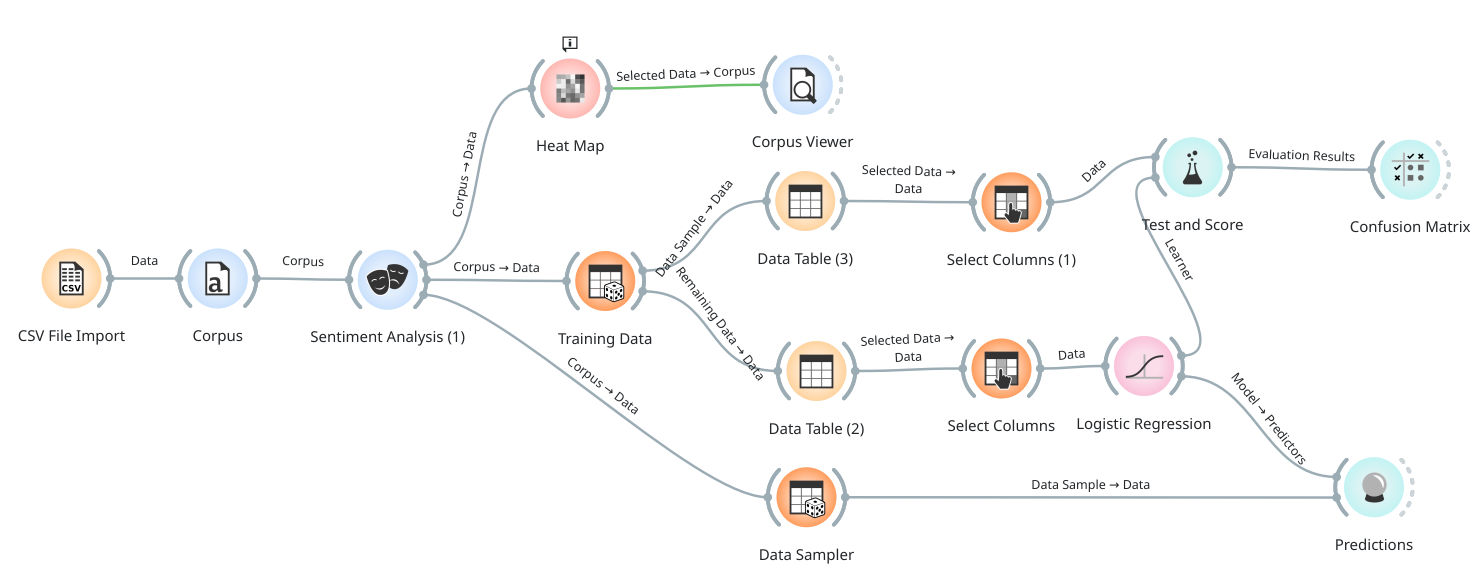
\includegraphics[width=\linewidth]{../figures/sentiment_pipeline.png}
	\caption{Pipeline untuk sentiment analysis menggunakan data Amazon dari UCI}
	\label{fig:sentiment-pipeline}
\end{figure}

\begin{enumerate}
	\item \textbf{CSV/Text File Import} \\
	Memuat dataset \texttt{amazon\_cells\_labelled.txt} (tab-delimited) yang berisi kolom teks ulasan dan label sentimen.
	
	\item \textbf{Corpus} \\
	Mengonversi data tabular menjadi \textit{Corpus}, memungkinkan pemrosesan teks lebih lanjut di Orange.
	
	\item \textbf{Sentiment Analysis} \\
	Menghitung skor sentimen (\textit{positive}, \textit{negative}, \textit{neutral}, dan \textit{compound}) per dokumen menggunakan pendekatan berbasis leksikon.
	
	\item \textbf{Heat Map} \\
	Visualisasi pola distribusi skor sentimen per dokumen dengan \textit{hierarchical clustering} untuk mengeksplor kemiripan ulasan.
	
	\item \textbf{Data Sampler → Training / Testing Data} \\
	Memisahkan data menjadi bagian pelatihan dan pengujian melalui widget \textit{Data Sampler}, sehingga dapat mengevaluasi model secara obyektif.
	
	\item \textbf{Select Columns} \\
	Memilih skor sentimen sebagai fitur, serta label sentimen sebagai target untuk pelatihan model.
	
	\item \textbf{Logistic Regression} \\
	Melatih model klasifikasi berdasarkan fitur skor sentimen.
	
	\item \textbf{Test \& Score} \\
	Mengevaluasi performa model terhadap data uji, menghasilkan metrik seperti:
	\begin{itemize}
		\item \textbf{CA} (Classification Accuracy),
		\item Precision, Recall, F1-score,
		\item AUC.
	\end{itemize}
	
	\item \textbf{Confusion Matrix} \\
	Menampilkan distribusi prediksi benar dan salah untuk tiap kategori sentimen.
	
	\item \textbf{Predictions} \\
	Menghasilkan dan menampilkan prediksi model untuk data baru atau diuji.
\end{enumerate}

\subsection*{Visualisasi Heatmap Skor Sentimen}

Gambar~\ref{fig:sentiment-heatmap} memperlihatkan hasil visualisasi \textit{heatmap} dari skor sentimen (\textit{positive}, \textit{negative}, \textit{neutral}, dan \textit{compound}) yang dihasilkan oleh widget \textit{Sentiment Analysis} untuk dataset Amazon.

Pada visualisasi ini:
\begin{itemize}
	\item Sumbu horizontal menunjukkan empat kategori skor sentimen:
	\begin{enumerate}
		\item \textbf{positive} — skor proporsi kata bernada positif dalam kalimat.
		\item \textbf{negative} — skor proporsi kata bernada negatif.
		\item \textbf{neutral} — skor proporsi kata netral.
		\item \textbf{compound} — skor gabungan dalam rentang $-1$ (sangat negatif) hingga $+1$ (sangat positif).
	\end{enumerate}
	
	\item Sumbu vertikal merepresentasikan setiap baris dokumen ulasan pada dataset, yang dikelompokkan secara hierarkis berdasarkan kemiripan profil skor sentimennya (\textit{hierarchical clustering}).
	
	\item Skala warna di bagian atas (biru $\rightarrow$ hijau $\rightarrow$ kuning) menunjukkan besar nilai skor:
	\begin{itemize}
		\item Biru = skor rendah atau negatif.
		\item Hijau = skor menengah.
		\item Kuning = skor tinggi atau positif.
	\end{itemize}
	
	\item Kotak hitam pada heatmap menandai kelompok dokumen yang memiliki pola skor sentimen yang serupa. Misalnya, pada kelompok yang ditandai, skor \textit{positive} dan \textit{neutral} relatif tinggi, sementara skor \textit{compound} rendah, yang mengindikasikan teks-teks tersebut mungkin mengandung campuran kata positif dan negatif sehingga skor akhir cenderung netral atau negatif.
\end{itemize}

Visualisasi seperti ini membantu dalam mengidentifikasi pola sentimen di antara ulasan, menemukan kelompok ulasan yang serupa, serta memberikan konteks tambahan sebelum data diproses ke tahap pelatihan model klasifikasi.

\begin{figure}[h]
	\centering
	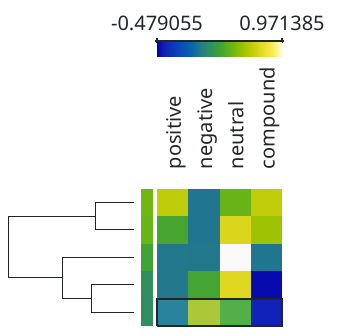
\includegraphics[width=0.5\linewidth]{../figures/sentiment_heatmap.png}
	\caption{Heatmap skor sentimen untuk dataset \texttt{amazon\_cells\_labelled.txt} dari UCI}
	\label{fig:sentiment-heatmap}
\end{figure}

\subsection*{Analisis Confusion Matrix}

Gambar~\ref{fig:sentiment-confmatrix} menunjukkan \textit{Confusion Matrix} hasil prediksi model \textit{Logistic Regression} terhadap dataset \texttt{amazon\_cells\_labelled.txt}. Confusion Matrix menampilkan distribusi jumlah prediksi benar dan salah untuk masing-masing kelas sentimen.

Pada matriks:
\begin{itemize}
	\item Baris merepresentasikan label \textbf{aktual} (ground truth).
	\item Kolom merepresentasikan label \textbf{prediksi} model.
	\item Kelas 0 = ulasan negatif, Kelas 1 = ulasan positif.
\end{itemize}

Hasil yang diperoleh:
\begin{itemize}
	\item \textbf{True Negative (TN)}: 45 ulasan negatif diprediksi benar sebagai negatif.
	\item \textbf{False Positive (FP)}: 5 ulasan negatif salah diprediksi sebagai positif.
	\item \textbf{False Negative (FN)}: 11 ulasan positif salah diprediksi sebagai negatif.
	\item \textbf{True Positive (TP)}: 39 ulasan positif diprediksi benar sebagai positif.
\end{itemize}

Interpretasi:
\begin{itemize}
	\item Model memiliki tingkat \textbf{akurasi} yang cukup tinggi, dengan mayoritas prediksi berada pada diagonal utama (TN dan TP).
	\item Hanya 16\% prediksi yang keliru (5 + 11 dari total 100 data uji).
	\item Kesalahan lebih banyak terjadi pada ulasan positif yang diklasifikasikan sebagai negatif (FN = 11) dibanding sebaliknya (FP = 5).
	\item Hal ini dapat mengindikasikan bahwa model sedikit lebih konservatif dalam memprediksi positif, atau beberapa ulasan positif mengandung kata-kata negatif yang kuat sehingga skor sentimennya bergeser.
\end{itemize}

\begin{figure}[h]
	\centering
	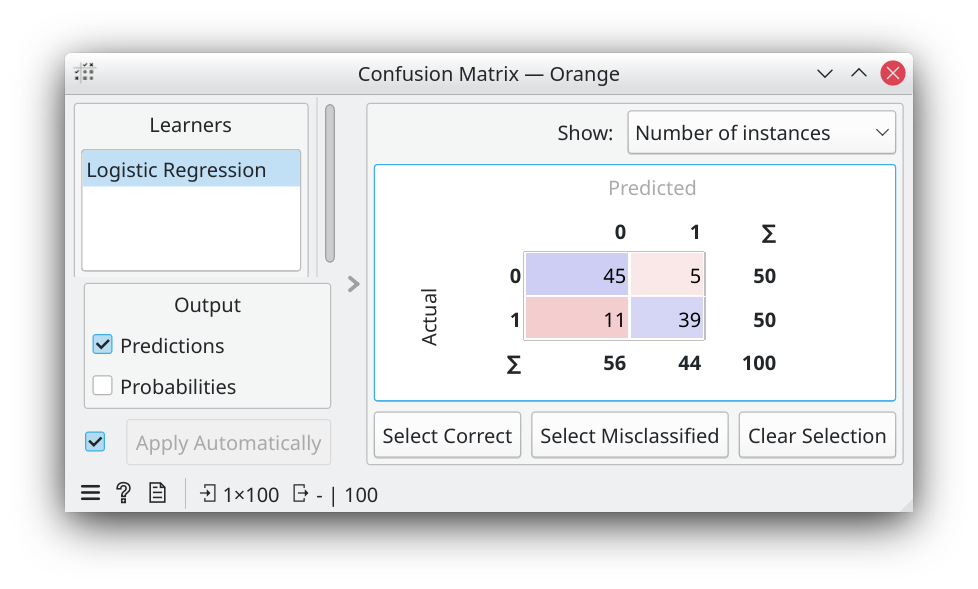
\includegraphics[width=0.6\linewidth]{../figures/sentiment_confusion_matrix.png}
	\caption{Confusion Matrix hasil prediksi Logistic Regression pada dataset \texttt{amazon\_cells\_labelled.txt}}
	\label{fig:sentiment-confmatrix}
\end{figure}


\subsection*{Evaluasi Model dengan Test and Score}

Evaluasi performa model klasifikasi dilakukan menggunakan widget \textit{Test and Score} pada Orange. Metode validasi yang digunakan adalah \textbf{cross-validation} dengan \textit{3-fold stratified}, yang memastikan distribusi kelas positif dan negatif seimbang di setiap fold pelatihan dan pengujian.

Gambar~\ref{fig:sentiment-testscore} menampilkan hasil evaluasi model \textit{Logistic Regression} terhadap dataset Amazon:

\begin{itemize}
	\item \textbf{AUC (Area Under Curve)} = 0.931 \\
	Menunjukkan kemampuan model membedakan kelas positif dan negatif. Nilai mendekati 1 berarti performa sangat baik.
	
	\item \textbf{CA (Classification Accuracy)} = 0.840 \\
	Persentase prediksi yang benar dari seluruh data uji, yaitu model berhasil mengklasifikasikan sekitar 84\% ulasan dengan benar.
	
	\item \textbf{F1-score} = 0.839 \\
	Rata-rata harmonis dari Precision dan Recall, merepresentasikan keseimbangan antara kedua metrik tersebut.
	
	\item \textbf{Precision} = 0.845 \\
	Proporsi prediksi positif yang benar-benar positif. Nilai ini menunjukkan sedikit di atas 84\% dari prediksi positif adalah benar.
	
	\item \textbf{Recall} = 0.840 \\
	Proporsi kasus positif yang berhasil dideteksi oleh model. Artinya, sekitar 84\% dari seluruh ulasan positif terklasifikasi dengan benar.
	
	\item \textbf{MCC (Matthews Correlation Coefficient)} = 0.685 \\
	Metrik korelasi antara prediksi dan label aktual, mempertimbangkan TP, TN, FP, dan FN. Nilai positif mendekati 1 menunjukkan korelasi yang kuat.
\end{itemize}

Dengan nilai AUC yang tinggi (0.931) dan akurasi yang stabil (0.840), dapat disimpulkan bahwa model Logistic Regression yang dibangun pada pipeline ini mampu mengklasifikasikan sentimen ulasan secara efektif pada dataset yang digunakan.

\begin{figure}[h]
	\centering
	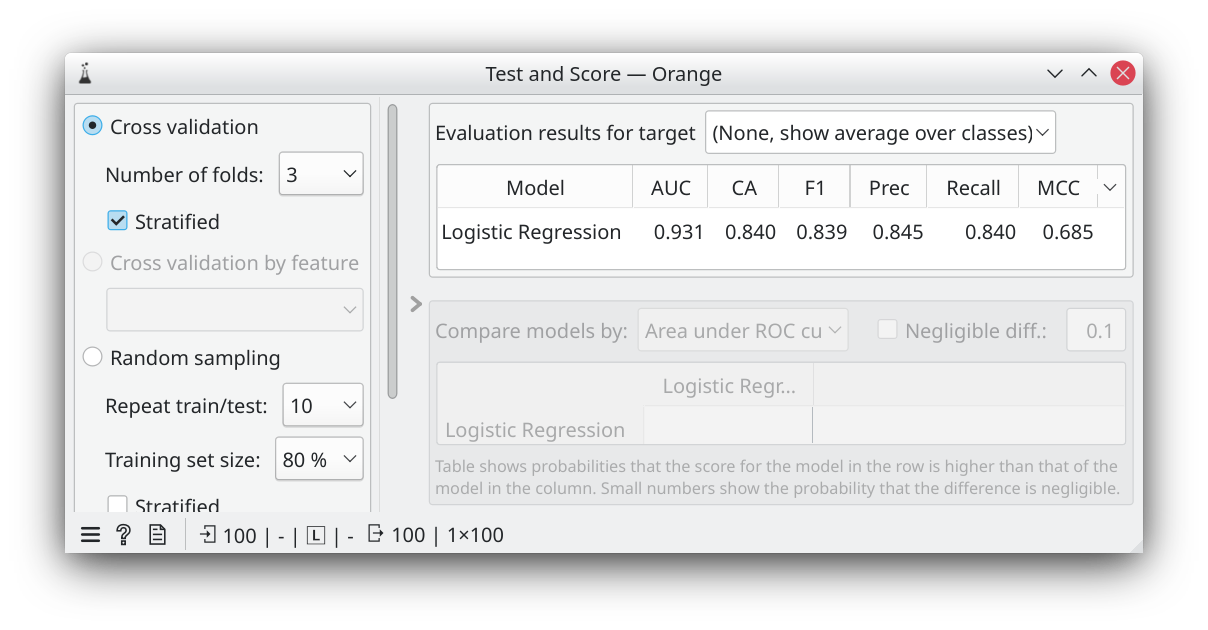
\includegraphics[width=0.75\linewidth]{../figures/sentiment_test.png}
	\caption{Hasil evaluasi model Logistic Regression menggunakan \textit{Test and Score} dengan 3-fold cross-validation pada dataset \texttt{amazon\_cells\_labelled.txt}}
	\label{fig:sentiment-testscore}
\end{figure}

\subsection*{Prediksi Sentimen pada Dataset}

Gambar~\ref{fig:sentiment-predictions} menampilkan keluaran dari widget \textit{Predictions} pada Orange, yang menunjukkan hasil prediksi model \textit{Logistic Regression} terhadap dataset \texttt{amazon\_cells\_labelled.txt}.

Widget \textit{Predictions} memberikan daftar label hasil prediksi untuk setiap entri teks dalam dataset, serta dapat menampilkan nilai probabilitas prediksi jika opsi tersebut diaktifkan. Pada kasus ini, tampilan memperlihatkan distribusi prediksi secara visual dalam bentuk warna untuk setiap baris data:
\begin{itemize}
	\item Setiap baris mewakili satu ulasan dari dataset.
	\item Warna mewakili kelas prediksi:
	\begin{itemize}
		\item Misalnya, oranye untuk prediksi \textbf{negatif} (0).
		\item Hijau untuk prediksi \textbf{positif} (1).
	\end{itemize}
	\item Urutan warna secara vertikal memperlihatkan urutan prediksi model terhadap keseluruhan dataset.
\end{itemize}

Dalam gambar, terlihat bahwa prediksi model tersebar antara kelas positif dan negatif, dengan pola warna yang relatif bervariasi. Hal ini menunjukkan bahwa dataset mengandung campuran ulasan positif dan negatif, serta model berhasil memisahkannya ke dalam dua kategori yang berbeda.

Widget ini berguna untuk:
\begin{itemize}
	\item Memeriksa hasil prediksi model terhadap data uji maupun data baru.
	\item Mengidentifikasi pola klasifikasi, misalnya jika terdapat bagian dataset yang didominasi oleh satu kelas tertentu.
	\item Mengekspor hasil prediksi untuk analisis lanjutan di luar Orange.
\end{itemize}

\begin{figure}[h]
	\centering
	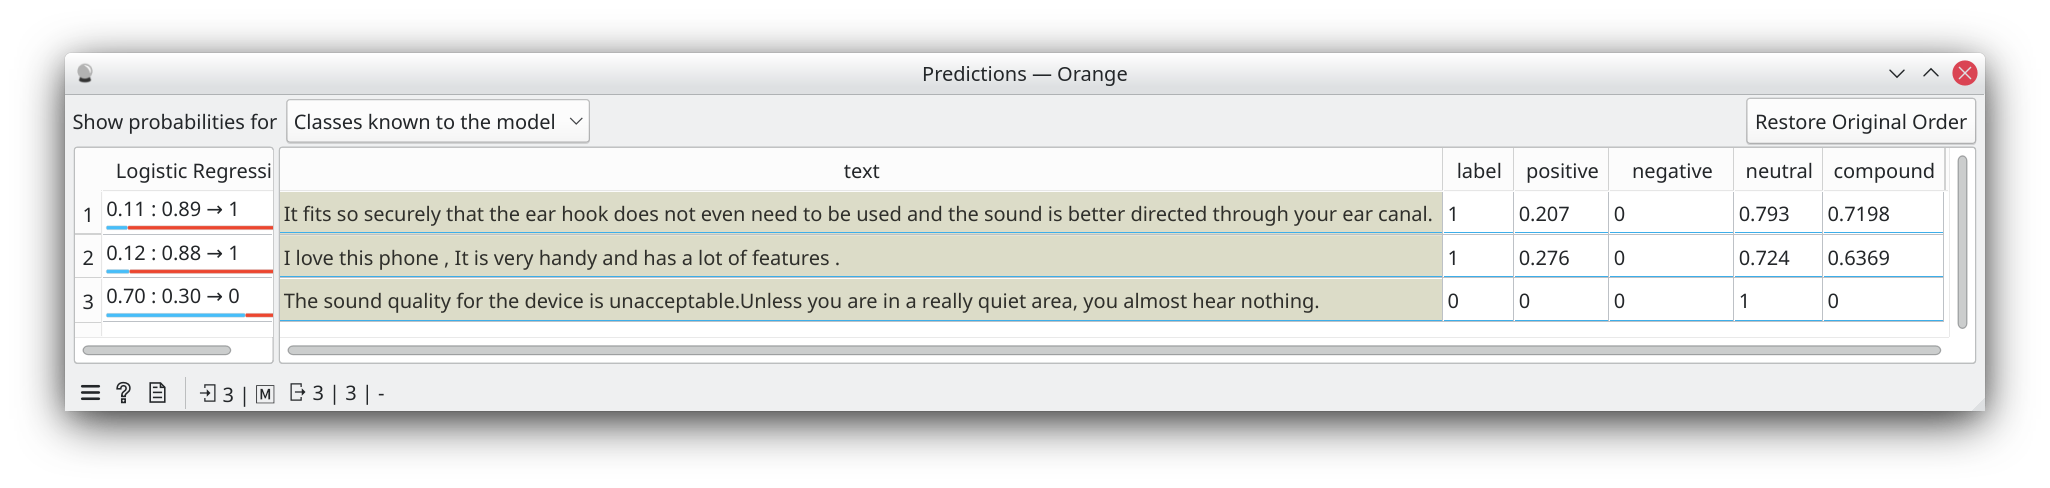
\includegraphics[width=\linewidth]{../figures/sentiment_prediction.png}
	\caption{Hasil prediksi model Logistic Regression terhadap dataset \texttt{amazon\_cells\_labelled.txt} ditampilkan menggunakan widget \textit{Predictions} di Orange}
	\label{fig:sentiment-predictions}
\end{figure}



\section{Interpretasi Hasil dan Strategi Bisnis}

Berdasarkan hasil analisis sentimen terhadap dataset \texttt{amazon\_cells\_labelled.txt} dari UCI Machine Learning Repository \cite{kotzias2015sentiment}, dapat disimpulkan beberapa temuan penting yang relevan untuk strategi bisnis.

\subsection*{Ringkasan Hasil Analisis}
\begin{itemize}
	\item \textbf{Heatmap Skor Sentimen} menunjukkan adanya kelompok ulasan dengan profil skor yang serupa, baik dari sisi skor positif, negatif, netral, maupun skor gabungan (\textit{compound}). Clustering ini dapat membantu mengidentifikasi segmen ulasan yang memiliki nuansa sentimen campuran, sehingga dapat dianalisis lebih lanjut untuk memahami faktor penyebabnya.
	\item \textbf{Evaluasi Model (Test and Score)} menghasilkan nilai AUC = 0.931, akurasi (CA) = 0.840, F1-score = 0.839, Precision = 0.845, dan Recall = 0.840. Nilai-nilai ini mengindikasikan bahwa model \textit{Logistic Regression} memiliki performa yang sangat baik dalam membedakan ulasan positif dan negatif pada dataset ini.
	\item \textbf{Confusion Matrix} memperlihatkan bahwa model melakukan prediksi benar pada 84\% data, dengan 45 ulasan negatif dan 39 ulasan positif terklasifikasi secara benar. Kesalahan lebih sering terjadi pada ulasan positif yang salah diprediksi sebagai negatif (FN = 11) dibandingkan sebaliknya (FP = 5).
	\item \textbf{Predictions} memperlihatkan distribusi prediksi positif dan negatif pada keseluruhan dataset, yang relatif seimbang. Hal ini mencerminkan distribusi kelas asli yang memang terdiri dari 50\% positif dan 50\% negatif.
\end{itemize}

\subsection*{Implikasi Strategi Bisnis}
Temuan di atas dapat diterjemahkan menjadi beberapa strategi bisnis yang aplikatif:
\begin{enumerate}
	\item \textbf{Pemantauan Kualitas Produk dan Layanan} \\
	Ulasan dengan skor sentimen negatif yang tinggi dapat diprioritaskan untuk dianalisis lebih lanjut. Kategori keluhan yang sering muncul dapat menjadi indikator area perbaikan, baik pada fitur produk maupun kualitas layanan pelanggan \cite{medhat2014sentiment}.
	\item \textbf{Peningkatan Retensi Pelanggan} \\
	Analisis pola pada ulasan positif yang konsisten dapat digunakan untuk mengidentifikasi faktor-faktor yang mendorong kepuasan pelanggan. Strategi retensi seperti program loyalitas dapat difokuskan pada aspek-aspek ini.
	\item \textbf{Segmentasi Pelanggan Berdasarkan Sentimen} \\
	Menggunakan hasil clustering dari heatmap, pelanggan dapat dikelompokkan ke dalam segmen sentimen spesifik (misalnya, sangat positif, campuran, atau sangat negatif). Setiap segmen dapat menerima komunikasi atau penawaran yang dipersonalisasi.
	\item \textbf{Pengukuran Dampak Perubahan Produk} \\
	Perubahan besar pada produk atau layanan (misalnya, peluncuran fitur baru) dapat dievaluasi dengan membandingkan distribusi sentimen sebelum dan sesudah implementasi \cite{liu2012sentiment}.
	\item \textbf{Integrasi dengan Sistem Otomatisasi} \\
	Model yang terlatih dapat diintegrasikan ke dalam sistem monitoring ulasan secara real-time untuk mendeteksi lonjakan sentimen negatif dan memberikan notifikasi cepat ke tim terkait.
\end{enumerate}

\subsection*{Keterbatasan dan Saran Pengembangan}
Walaupun model menunjukkan performa tinggi, beberapa keterbatasan tetap ada:
\begin{itemize}
	\item Dataset relatif kecil (1.000 ulasan) dan homogen (hanya produk ponsel dari Amazon), sehingga generalisasi ke domain lain perlu diuji.
	\item Analisis sentimen berbasis leksikon dapat kurang akurat untuk mendeteksi sarkasme, ironi, atau konteks bahasa yang kompleks \cite{pang2008opinion}.
	\item Model hanya mengklasifikasikan ke dalam dua kelas (positif dan negatif), padahal dalam praktik bisnis, kategori netral atau nuansa sentimen yang lebih halus juga penting.
\end{itemize}

Pengembangan selanjutnya dapat mencakup:
\begin{itemize}
	\item Menggunakan dataset yang lebih besar dan beragam.
	\item Mengadopsi model berbasis \textit{deep learning} seperti BERT untuk menangkap konteks kalimat yang lebih kompleks.
	\item Menambahkan analisis topik (\textit{topic modeling}) untuk memahami tema utama yang sering muncul pada ulasan dengan sentimen tertentu.
\end{itemize}

Dengan interpretasi hasil yang tepat, analisis sentimen seperti ini dapat menjadi landasan penting dalam pengambilan keputusan strategis, membantu bisnis untuk merespons masukan pelanggan secara proaktif, dan meningkatkan daya saing di pasar.


\section{Penutup}
Keseluruhan pembahasan menunjukkan bahwa analisis teks dan sentimen merupakan komponen penting dalam pemrosesan bahasa alami yang mampu mengubah data teks tidak terstruktur menjadi wawasan strategis. Mulai dari tahap pengumpulan dan prapemrosesan data, ekstraksi fitur, hingga pemilihan metode klasifikasi, setiap langkah memiliki peran krusial dalam menghasilkan model yang akurat. Beragam pendekatan—mulai dari berbasis kamus, pembelajaran mesin, hingga pembelajaran mendalam—menawarkan keunggulan dan keterbatasannya masing-masing, sehingga pemilihan metode harus mempertimbangkan tujuan analisis, ketersediaan data, serta sumber daya komputasi. Studi kasus ulasan produk e-commerce menegaskan bagaimana analisis sentimen dapat membantu mengidentifikasi pola persepsi pelanggan secara kuantitatif, sekaligus memandu strategi perbaikan dan inovasi.

Hasil implementasi menggunakan dataset publik Amazon dan alat visual Orange menunjukkan performa model yang tinggi, dengan AUC mencapai 0.931 dan akurasi 84\%. Visualisasi seperti heatmap dan confusion matrix memperkaya pemahaman terhadap distribusi sentimen serta pola kesalahan prediksi. Implikasi bisnis dari temuan ini sangat luas, mulai dari pemantauan kualitas produk, peningkatan retensi pelanggan, hingga segmentasi berbasis sentimen. Meskipun terdapat keterbatasan, seperti ukuran dataset yang kecil dan domain yang spesifik, pendekatan ini tetap menawarkan fondasi yang kuat bagi pengambilan keputusan berbasis data. Dengan pengembangan lebih lanjut, termasuk penggunaan model kontekstual seperti BERT dan dataset yang lebih beragam, analisis sentimen dapat menjadi alat prediktif dan diagnostik yang semakin andal dalam ekosistem bisnis modern.